\documentclass{beamer}
\usepackage{listings}

\newcommand{\bd}{\begin{description}} 
\newcommand{\ed}{\end{description}} 
\newcommand{\bi}{\begin{itemize}} 
\newcommand{\ei}{\end{itemize}} 


\title{MATH12345 Scientific Computing \\ Analysis Exercise 0}
\subtitle{The Fibonacci sequence}
\author{Joe Cool \\ Student ID: 12345}
%\date{\tiny Please update course code, project number, name and Student ID!}
\begin{document}


%%%%%%%%%%%%%%%%%%%%%%%%%%%%%%%%%%%%%%%%%%%%%%%%%%%%%%%%%%%%%%%%%%%%%%

\frame{\titlepage}

%%%%%%%%%%%%%%%%%%%%%%%%%%%%%%%%%%%%%%%%%%%%%%%%%%%%%%%%%%%%%%%%%%%%%%

\begin{frame}
  \frametitle{The Fibonacci sequence}
  \begin{overlayarea}{\textwidth}{\textheight}
    
    \bi
  \item The Fibonacci sequence is defined by
    \begin{align}
      f_0 &= 1,\\\quad f_1 &= 1,\\\quad f_n &= f_{n-1} + f_{n-2}\quad\text{for}\quad n\geq 2.
    \end{align}
  \item Aim: compute the sequence $f_{n} \ (n=0,1,2,...)$ by the
    recursive definition given above and compare against a known explict
    expression for the $n$-th value.
    
  \item Implementation:
    \bi
  \item Straightforward loop to find 
    $f_n$, from $f_{n-1}$ and $f_{n-2}$,
    following the initialisation of $f_0$ and $f_1$.
  \item Only need to store $f_{n-1}$ and $f_{n-2}$ in temporary
    variables. No need to keep track of the entire sequence.
    \ei
    \ei
    
  \end{overlayarea}
\end{frame}

%%%%%%%%%%%%%%%%%%%%%%%%%%%%%%%%%%%%%%%%%%%%%%%%%%%%%%%%%%%%%%%%%%%%%%

\begin{frame}
  \frametitle{The Fibonacci sequence}
  \begin{overlayarea}{\textwidth}{\textheight}
    
    \vspace{0.5cm}
           {\bf Result:} Plot of $f_n$ vs. $n$:
           \begin{center}
             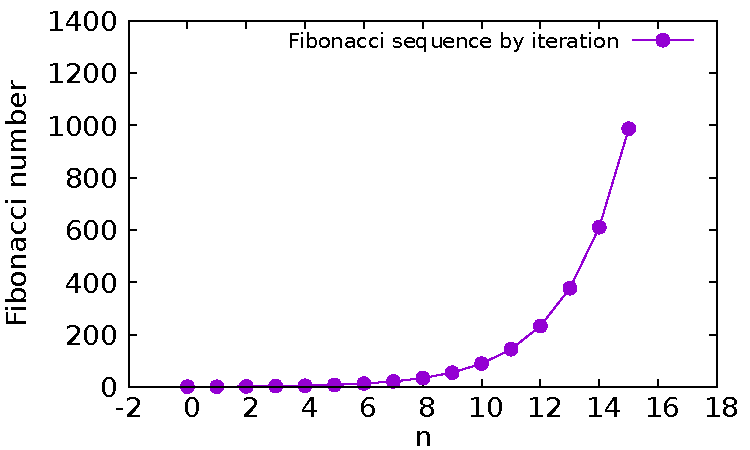
\includegraphics[width=10cm]{code/fibonacci.pdf}
           \end{center}
           
  \end{overlayarea}
\end{frame}

%%%%%%%%%%%%%%%%%%%%%%%%%%%%%%%%%%%%%%%%%%%%%%%%%%%%%%%%%%%%%%%%%%%%%%


\begin{frame}
  \frametitle{The Fibonacci sequence: Validation (i)}
  \begin{overlayarea}{\textwidth}{\textheight}
    
    A basic validation is to check that
    each value is the sum of the previous two. Outputting $n, f_n$ for
    the first few values of $n$ yields
    \begin{center}
    \scalebox{0.8}{
      \lstinputlisting[linerange={1-12}]{code/n_fn.dat}
    }
    \end{center}
    That seems correct for the first twelve values computed.

    \vspace{1cm}
    \scriptsize
    [Note: Generally, displaying ``raw'' numbers or screenshots of a
      code's output is a bad idea! Use graphical representations.]
\end{overlayarea}
\end{frame}
%%%%%%%%%%%%%%%%%%%%%%%%%%%%%%%%%%%%%%%%%%%%%%%%%%%%%%%%%%%%%%%%%%%%%%


\begin{frame}
  \frametitle{The Fibonacci sequence: Validation (ii)}
  \begin{overlayarea}{\textwidth}{\textheight}

    \small 
    We can also exploit that an explicit expression for the $n$-th
    Fibonacci number is known (e.g. using the Wikipedia reference
    provided):
    $$
    f_n = \frac{\phi^{n+1}-\psi^{n+1}}{\phi-\psi},
    $$
    where $\psi = -1/\phi = (1-\sqrt{5})/2$. (Note the offset in the
    index compared to the result given on Wikipedia!)

    \vspace{0.3cm}

    {\bf Result:} Plot of $f_n$ vs. $n$, using the result from the
    code (filled circle) and from the explicit expression (square):
    They agree! 
    \begin{center}
      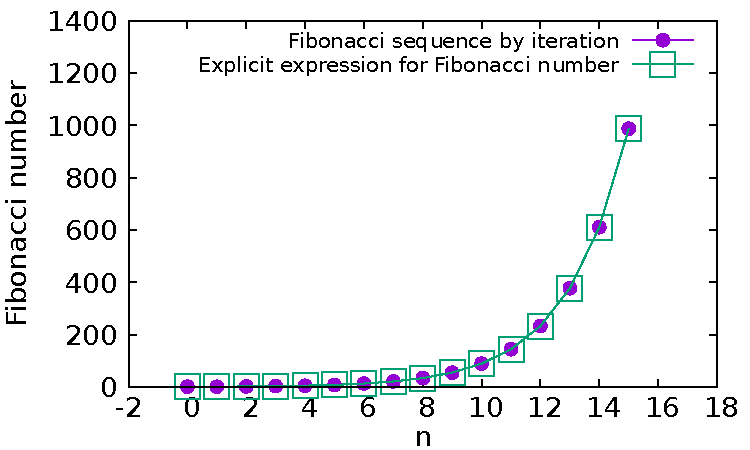
\includegraphics[width=6cm]{code/fibonacci_validation.pdf}
    \end{center}

\end{overlayarea}
\end{frame}

%%%%%%%%%%%%%%%%%%%%%%%%%%%%%%%%%%%%%%%%%%%%%%%%%%%%%%%%%%%%%%%%%%%%%%

\end{document}


